\documentclass[a4paper]{article}
\usepackage[francais]{babel}
\usepackage[utf8]{inputenc}

\usepackage{graphicx}
\usepackage{fancyhdr}
\usepackage{lastpage}
\usepackage{amsmath}
\usepackage{xspace}
\usepackage{textcomp}

\usepackage{hyperref}

\usepackage[top=30mm, bottom=30mm, left=25mm, right=25mm]{geometry}

\pagestyle{fancy}

\usepackage{helvet}
\usepackage{bbm}

\usepackage{verbatim}
\usepackage{amsmath}
\usepackage[table]{xcolor}
\definecolor{bleugris}{rgb}{.2,.4,.5}

\definecolor{colKeys}{rgb}{0,0,1} 
\definecolor{colIdentifier}{rgb}{0,0,0} 
\definecolor{colComments}{rgb}{0,0.5,1} 
\definecolor{colString}{rgb}{0.6,0.1,0.1} 

\usepackage{listings}

% Permet l'ajout de code par insertion du fichier le contenant
% Les arguments sont :
% $1 : nom du fichier � inclure
% $2 : le type de langage (C++, C, Java ...)
\newcommand{\addCode}[2]{%

  % Configuration de la coloration syntaxique du code
  \definecolor{colKeys}{rgb}{0,0,1}
  \definecolor{colIdentifier}{rgb}{0,0,0}
  \definecolor{colComments}{rgb}{0,0.5,1}
  \definecolor{colString}{rgb}{0.6,0.1,0.1}

  % Configuration des options 
  \lstset{%
    language = #2,%
    identifierstyle=\color{colIdentifier},%
    basicstyle=\ttfamily\scriptsize, %
    keywordstyle=\color{colKeys},%
    stringstyle=\color{colString},%
    commentstyle=\color{colComments},%
    columns = flexible,%
    %tabsize = 8,%
    showspaces = false,%
    numbers = left, numberstyle=\tiny,%
    frame = single,frameround=tttt,%
    breaklines = true, breakautoindent = true,%
    captionpos = b,%
    xrightmargin=10mm, xleftmargin = 15mm, framexleftmargin = 7mm,%
  }%
    \begin{center}
    \lstinputlisting{#1}
    \end{center}
}

\newcommand{\nTitle}[1]{%
	\clearpage
	\vspace*{\fill}		%
	\begin{center}	%
		\part{#1}		%
	\end{center}
	\vspace*{\fill}		%
	\clearpage
}

\newenvironment{nAbstract} 		%
{ 								%
	\newpage 					% 
	\vspace*{\fill}				%
	\begin{center}			 	%
		\begin{abstract}		%
}{								%
		\end{abstract}			%
	\end{center}				%
	\vspace*{\fill}				%
	\newpage					%
}


\newcommand{\nClass}[1]{{\color{bleugris}{\textsl{\textbf{#1}}}}}
\newcommand{\nParameter}[1]{{\color{gray}{\textbf{#1}}}}
\newcommand{\nMethod}[1]{{\color{gray}{\textbf{#1}}}}
\newcommand{\nConstant}[1]{\texttt{\uppercase{#1}}}
\newcommand{\nKeyword}[1]{\textsl{\textbf{#1}}}

\graphicspath{{../SourcesMatlab/}}

% Conversion nombres arabes / romain
\makeatletter
\newcommand{\rmnum}[1]{\romannumeral #1}
\newcommand{\Rmnum}[1]{\expandafter\@slowromancap\romannumeral #1@}
\makeatother

\setlength{\headheight}{14pt}

\fancyhf{}


\makeatletter
\def\clap#1{\hbox to 0pt{\hss #1\hss}}%
\def\ligne#1{%
\hbox to \hsize{%
\vbox{\centering #1}}}%
\def\haut#1#2#3{%
\hbox to \hsize{%
\rlap{\vtop{\raggedright #1}}%
\hss
\clap{\vtop{\centering #2}}%
\hss
\llap{\vtop{\raggedleft #3}}}}%
\def\bas#1#2#3{%
\hbox to \hsize{%
\rlap{\vbox{\raggedright #1}}%
\hss
\clap{\vbox{\centering #2}}%
\hss
\llap{\vbox{\raggedleft #3}}}}%
\def\maketitle{%
\thispagestyle{empty}\vbox to \vsize{%
\vfill
\vspace{1cm}
\begin{flushleft}
\usefont{OT1}{ptm}{m}{n}
\huge \@title
\end{flushleft}
\par
\hrule height 4pt
\par
\begin{flushright}
\usefont{OT1}{phv}{m}{n}
\Large \@author
\par
\end{flushright}
\vspace{1cm}
\vfill
\vfill
\bas{}{\@blurb \vspace{1cm}}{}
}%
\cleardoublepage
}
\def\date#1{\def\@date{#1}}
\def\author#1{\def\@author{#1}}
\def\title#1{\def\@title{#1}}
\def\blurb#1{\def\@blurb{#1}}
\author{}
\title{}
\blurb{}
\makeatother

\usepackage{hyperref}
\hypersetup{
colorlinks=false, % bool: Liens colorés
pdfborder={0 0 0} % Ne pas encadrer les liens
}

\usepackage[final]{pdfpages}
\usepackage{rotating}
\usepackage{eurosym}
\usepackage{lscape}
\usepackage{float}
\usepackage{color}
\usepackage{colortbl}
\usepackage{array}
\usepackage[printonlyused]{acronym}

% définir les commandes ici

% s'il y a beaucoup de commandes et de packages à inclure n'h&ésitez pas
% à mettre tout ça dans un fichier include.tex et l'inclure
% \input{include.tex}

\lhead{PdC2 - Dossier d'Architecture}
\rhead{
\includegraphics [width=1.5cm]{insa-couleur.jpg}}
\rfoot{\thepage\ de \pageref{LastPage}}



\begin{document}
\title{PdC 9 : Environement Technico-pédagogique}
\author{Adrien Brochot, Julien Levesy, Martin Richard, Armand Rossius}

%------------------------------------- Page de titre
\maketitle
%\begin{titlepage}
%~

%\vfill
%\begin{Large}
%Septembre 2011
%\end{Large}
%\vfill
%\end{titlepage}
%----------------------------------------------------

%--------------------------------- Table des matières
\newpage
\tableofcontents
\newpage
%----------------------------------------------- Plan
\newpage
\section*{Introduction}

L’objectif de ce document est de présenter les différents cas d’utilisation de la plateforme pédagogique que nous proposons de mettre en place.\\

Il doit permettre de résumer de manière claire et synthétique les différents usages possible de la solution que nous proposons par les différents acteurs intervenant dans le cadre de celle-ci.\\

Ces différents cas d’utilisation permettrons de définir de manière claire les besoins fonctionnels de la solution proposée.\\

Nous présenterons dans un premier temps un schéma global d’utilisation de la plateforme pédagogique, puis nous étudierons plus en détails les cas d’utilisation à l’aide de 4 autres diagramme de cas d’utilisation.\\

%\newpage
\section{CU1 - Diagramme général}

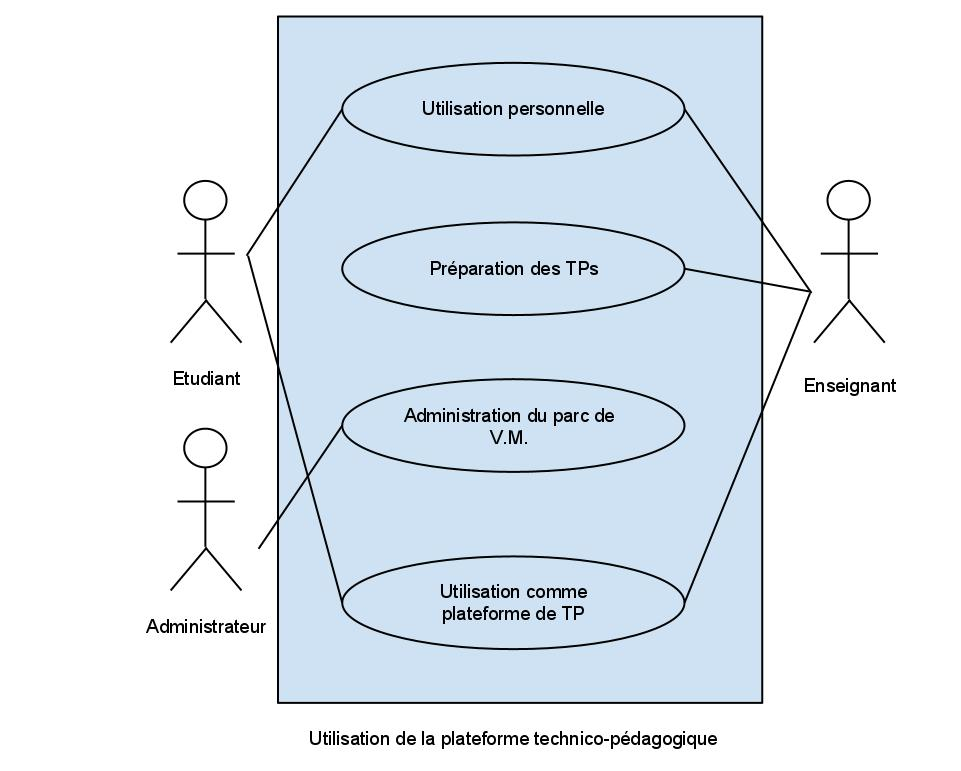
\includegraphics[scale=0.4]{CU1.jpg}

Dans l’organisation générale de cet outil pédagogique, nous pouvons identifier différents acteurs. Il y a tout d’abord l’étudiant, au coeur du système : il a la possibilité de s’identifier et d’utiliser les Machines Virtuelles mises à sa disposition. L’enseignant possède dans cet outil les mêmes cas d’utilisation de base que les étudiant. Il peut en outre utiliser la plate-forme mise à sa disposition pour préparer des travaux pratiques spécifiques et fournir des machines virtuelles de travail aux étudiants. Enfin, le dernier acteur utilisant ce produit est l’administrateur : Il a la possibilité d’administrer le parc de machines virtuelles.


\section{CU2 - Utilisation personnelle}

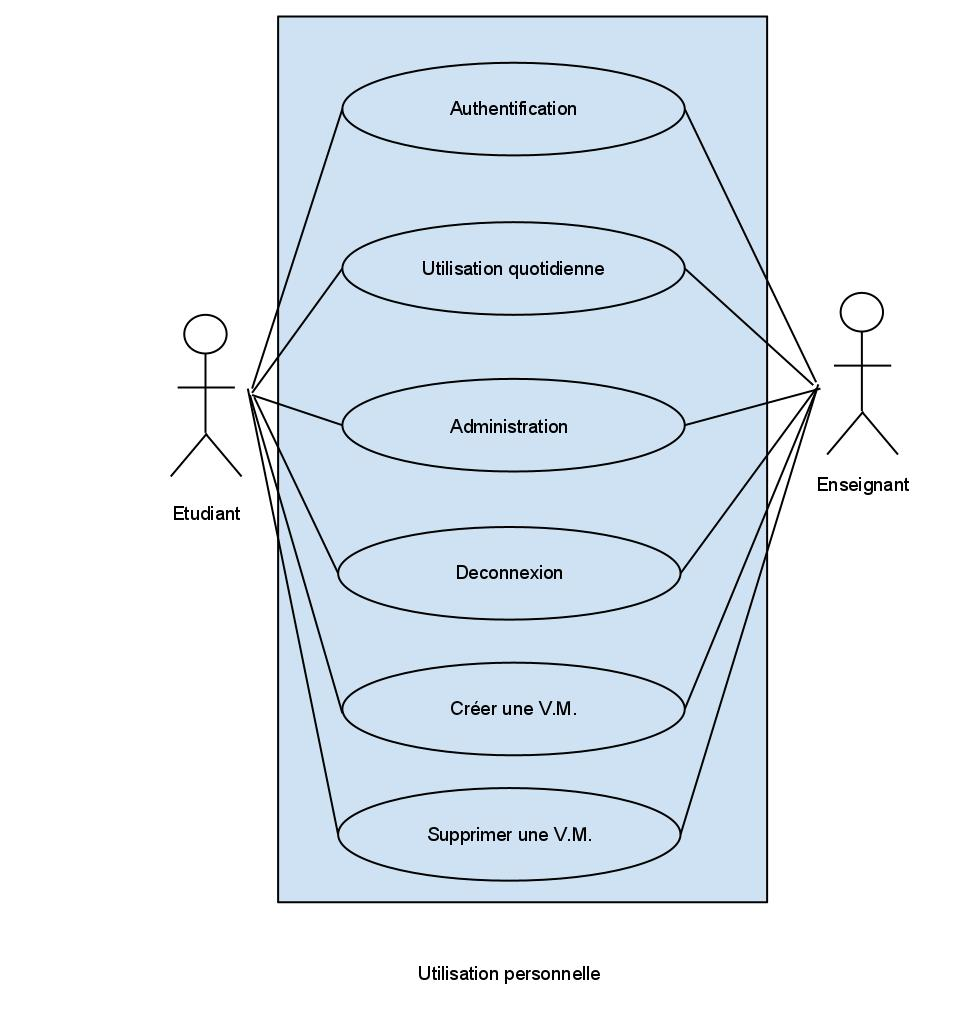
\includegraphics[scale=0.4]{CU2.jpg}

Le but des machines virtuelles est à terme de remplacer le système de session utilisées à l’I.N.S.A.
En terme d’utilisation personnelle, l’enseignant et l’étudiant auraient les mêmes possibilités.

Pour utiliser une machine virtuelle, l’utilisateur (étudiant ou enseignant) devra tout d’abord se connecter (\underline{authentification}). Ensuite, il sera libre d’utiliser sa machine virtuelle afin d’en faire une \underline{utilisation quotidienne} (naviguer sur internet, utiliser des applications, consulter ses e-mails, etc...). Il aura également la possibilité d’effectuer des tâches d’\underline{administration} sur sa machine.

Puisque chaque utilisateur dispose d’un quota pour gérer ses machines virtuelles, il a également la possibilité de créer une nouvelle machine virtuelle (\underline{créer une V.M.}), ou d’en supprimer une existante (\underline{supprimer une V.M.}).

Enfin, l’utilisateur devra enfin lorsqu’il aura cessé d’utiliser une machine virtuelle, utiliser la fonction de \underline{déconnexion}.


\section{CU3 - Préparation des machines de TPs}

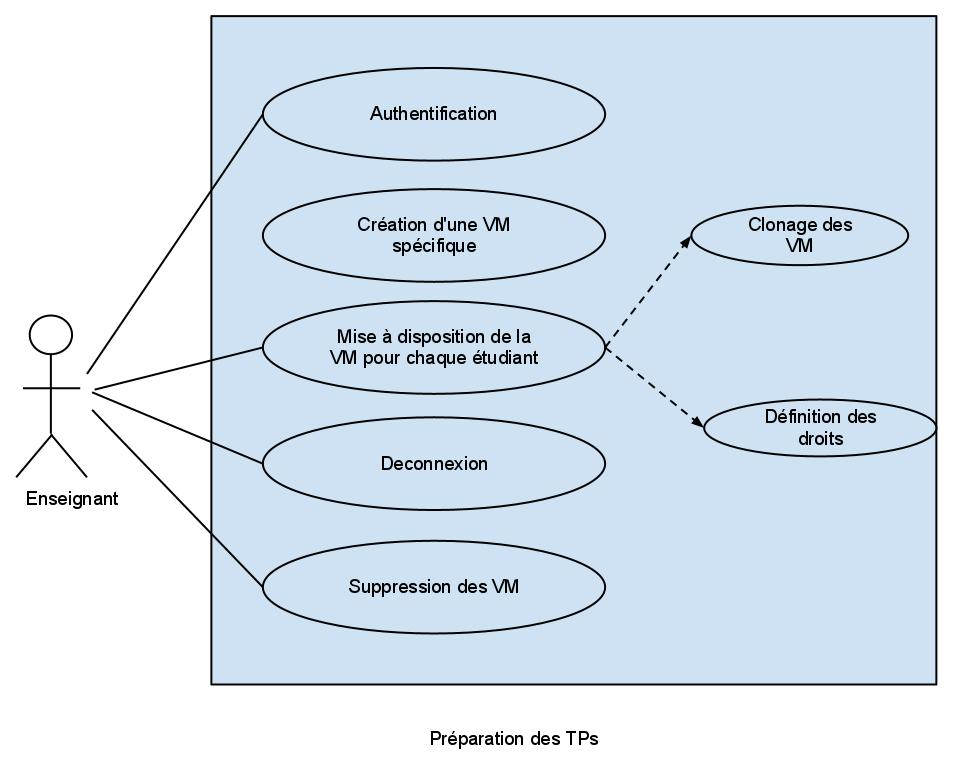
\includegraphics[scale=0.4]{CU3.jpg}

L’un des principaux avantages de cet outil technopédagogique est la souplesse qu’il procure dans la création et la diffusion de machines personnalisées pour des tâches spécifiques. Ainsi, il est très facile à un enseignant de créer des machines virtuelles spécialement pour un projet et de les fournir aux étudiants afin qu’ils puissent réaliser le travail demandé.
Au coeur de ce cas d’utilisation se trouve l’enseignant qui, en s’authentifiant sur le serveur d’infrastructure aura accès à une parc de machines virtuelles configurables. Il pourra alors en cloner une et la personnaliser afin de préparer les outils nécessaires à la réalisation du projet qu’il envisage de proposer aux étudiants. Une fois la machine prète, il lui sera également très aisé de la cloner de multiples fois afin d’en avoir suffisamment de copies pour tous les groupes d’étudiants. Il peut alors modifier les droits afin de restreindre l’accès aux machines de travail et permettre aux étudiants de travailler dans des conditions optimales. Suite à réalisation du travail par les étudiants (dont le déroulement est décrit en CU4), l’enseignant pourra supprimer les machines virtuelles de travail après correction.

\section{CU4 - Utilisation comme plateforme de TPs}

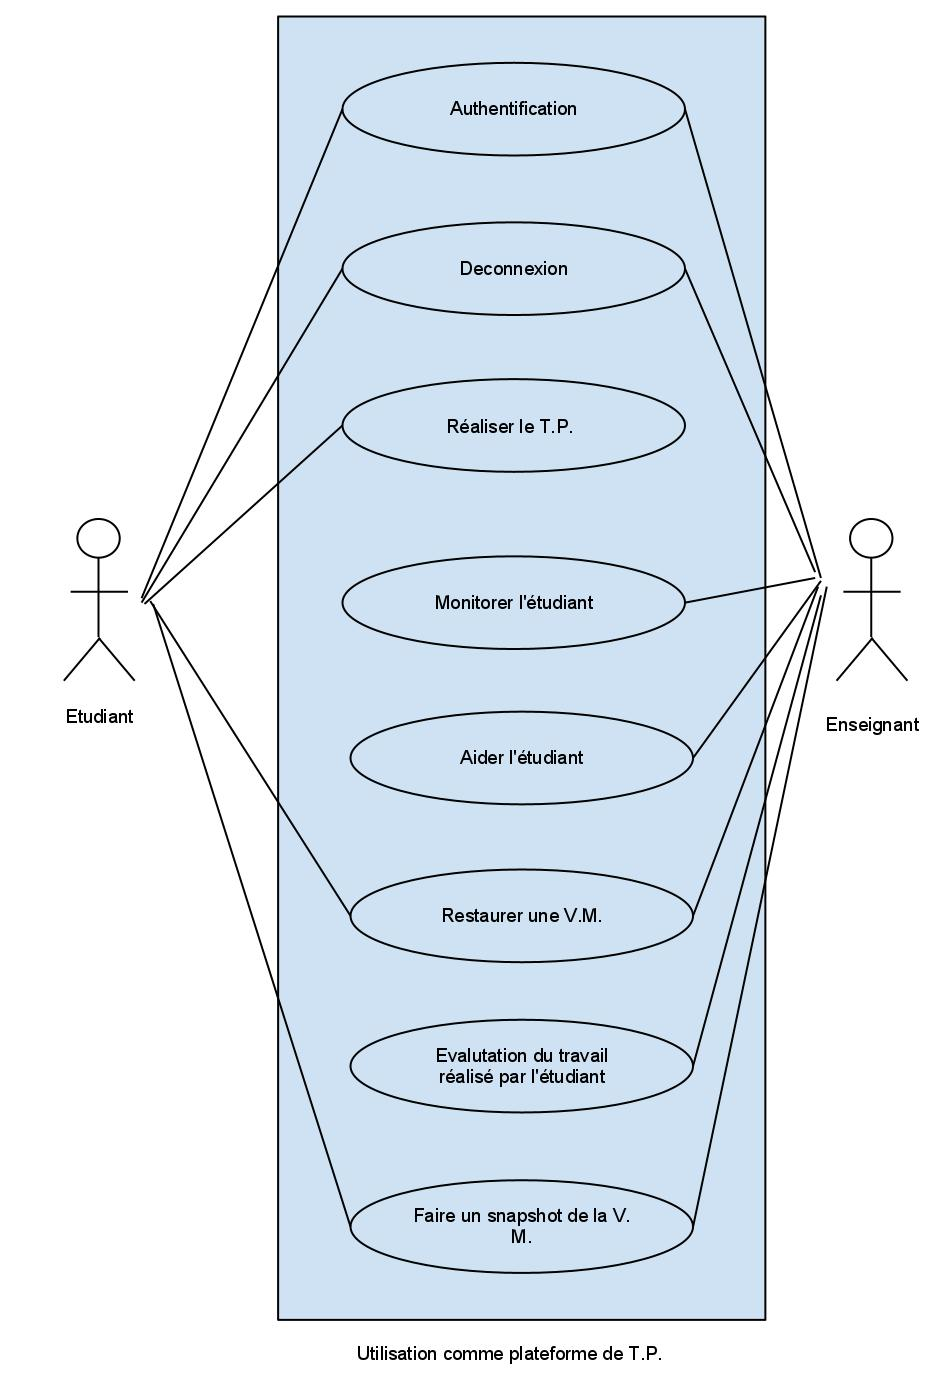
\includegraphics[scale=0.4]{CU4.jpg}

L’un des objectifs pédagogiques de la solution est de pouvoir réaliser des plateformes de T.P. axées autour de l’utilisation des machines virtuelles.

L’étudiant (et l’enseignant) doit tout d’abord se connecter (\underline{authentification}) pour pouvoir utiliser la machine virtuelle du T.P.
L’étudiant réalise ensuite le travail demandé pour le T.P. (\underline{réaliser le T.P.}). Pendant ce temps, l’enseignant a la possibilité de \underline{monitorer l’étudiant}, et de l’aider si besoin (\underline{aider l’étudiant}).

L’étudiant (ainsi que l’enseignant) a la possibilité \underline{faire un snapshot de la V.M.}, et d’effectuer un backup de l’état de la machine (\underline{restaurer une V.M.}).

L’enseignant pourra ensuite \underline{évaluer le travail de l’étudiant}.

Enfin, l’étudiant (ainsi que l’enseignant) devra \underline{se déconnecter} de la machine virtuelle.

\section{CU5 - Administration du parc de V.M.}

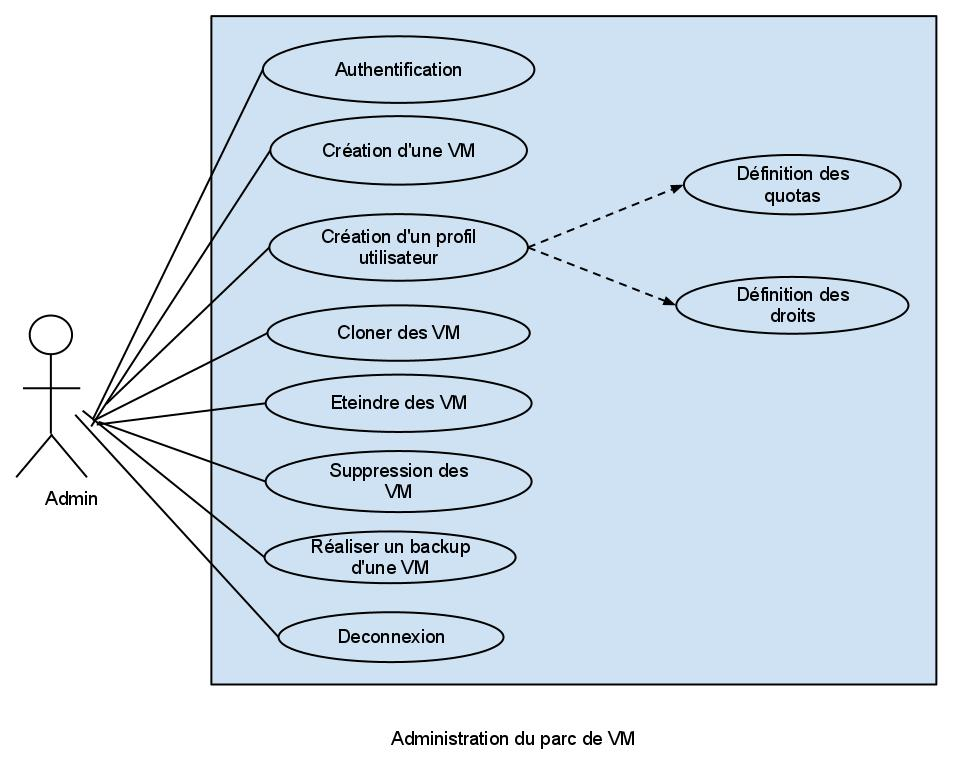
\includegraphics[scale=0.4]{CU5.jpg}

L’administrateur du système devra tout au long de l’année veiller à ce que la plateforme reste exploitable malgré la création/suppression constante de machines virtuelles pour les différents travaux pratique. Sa première tâche sera de créer et mettre à disposition des étudiants ainsi que des enseignants des machines virtuelles de base possédant une configuration minimale laissant les utilisateurs libres de les cloner pour les personnaliser. Il aura également pour rôle de définir les droits d’accès aux différents répertoires de machines virtuelles aux utilisateurs en fonction de leur groupe ou status. 
La sauvegarde de certaines machines sera également dans ses attributions car la perte de certaines machines critiques pourrait grandement pénaliser l’enseignement au département en cas de défaillance du serveur principal.
Il pourra enfin supprimer les machines virtuelles inutiles ou possédée par des utilisateur n’étudiant plus au département.

\end{document}